\documentclass[tikz]{standalone}
\usepackage{mymacros}
\usetikzlibrary{positioning} % for below of
\begin{document}
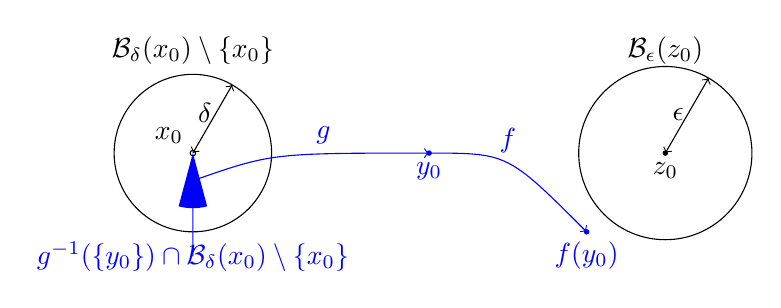
\begin{tikzpicture}
  \coordinate (x0) at (0,0);
  \draw (x0) circle (1);
  \node [above=of x0]
    {$\mathcal{B}_\delta (\vect{x}_0)\setminus\left\{\vect{x}_0\right\}$};
  \draw [fill=white] (x0) circle (1pt)
    node [above left] {$\vect{x}_0$}; % label on top
  \coordinate (centroid) at (0,-0.35);
  \fill [blue] (x0) -- (255:0.7) arc (255:285:0.7)
  coordinate [pos=0.5] (x0s) -- cycle;
  \node [color=blue,below=of x0] (lbl1)
    {$g^{-1} (\left\{\vect{y}_0\right\}) \cap \mathcal{B}_\delta (\vect{x}_0)
    \setminus \left\{ \vect{x}_0 \right\}$};
  \draw[<->] (x0) -- ++(60:1) node[pos=.3,above] {$\delta$};
  \coordinate (y0) at (3,0);
  \draw [color=blue] (lbl1.center) -- (x0s);
  \draw [color=blue,->] (centroid) .. controls(1,0) .. (y0)
    node [pos=0.7,above] {$g$};
  \fill [blue] (y0) circle (1pt) node [below] {$\vect{y}_0$}; % label
  \coordinate (z0) at (6,0);
  \draw (z0) circle (1.1);
  \node [above=of z0] {$\mathcal{B}_\epsilon (\vect{z}_0)$};
  \fill (z0) circle (1pt) node [below] {$\vect{z}_0$};
  \draw[<->] (z0) -- ++(60:1.1) node[pos=.3,above] {$\epsilon$};
  \coordinate [below left=of z0] (fy0);
  \fill [blue] (fy0) circle (1pt) node [below] {$f(\vect{y}_0)$};
  \draw[color=blue,->] (y0) .. controls(4,0) .. (fy0)
  node [pos=.5,above] {$f$};
\end{tikzpicture}
\end{document}
